\documentclass[aspectratio=1610]{beamer}

\usepackage{transparent}
% \definecolor{links}{HTML}{FF0000}
% \hypersetup{colorlinks,linkcolor=links,urlcolor=links}

\usetheme{Copenhagen}

\title[Student Engineer Design Portfolio]{Design Portfolio}
\subtitle{ESC102 Praxis II}
\author[Page \insertframenumber]{Kevin (Zerui) Wang}
\institute{University of Toronto}
\date{\today}

\begin{document}
{
\setbeamertemplate{footline}{}
\begin{frame}
\titlepage
\end{frame}
}
\addtocounter{framenumber}{-1}

{
% \setbeamertemplate{background}{
%     
\includegraphics[width=\paperwidth,height=\paperheight]{images/portfolio.jpg}
% }
\begin{frame}{Table of Contents}
    \tableofcontents
\end{frame}
}

\section{Egineering, Design, and Engineering Design}

\section{Position in Context}
\subsection{Values}

\begin{frame}
   AMONG US
   \begin{enumerate}[I]
    \item red sus
    \item cyan sus
    \begin{enumerate}[i]
    \item red vented
    \item emergency meeting
    \end{enumerate}
    \item moyai
    \item red ejected
    \end{enumerate}
\end{frame}
\subsection{Abilities}
\subsection{Strengths}
\subsection{Biases}
\subsection{Areas for Improvement}

\section{Design Experiences}
\subsection{Praxis I}
\subsection{CIV102 Bridge}
\subsection{Praxis II}

{
% \setbeamertemplate{background}{
%     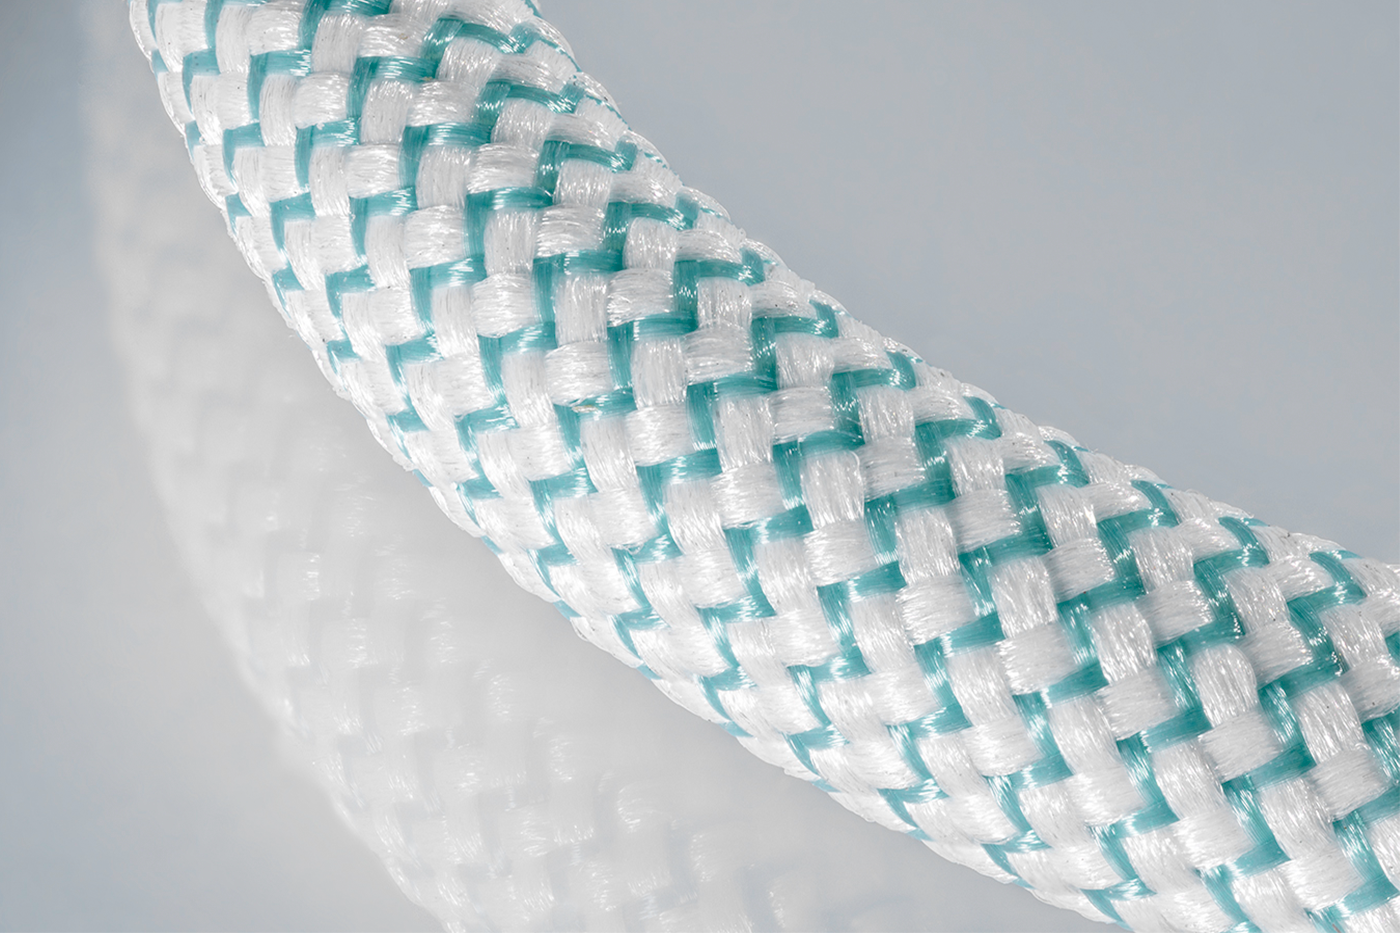
\includegraphics[width=\paperwidth,height=\paperheight]{images/braid.png}
% }
\begin{frame}{Monkey}
    :moyai:
\end{frame}
}

\begin{frame}
    \frametitle{Title}
    lorem dolor sit amet
\end{frame}

\begin{frame}
    \frametitle{Title}
    lorem dolor sit amet
\end{frame}

\begin{frame}{Title deez}

\end{frame}

\begin{frame}{b}{ruh}
    ayoooooooooo

\end{frame}

\end{document}